\documentclass[a4paper]{article}
\usepackage{graphicx, color}
\usepackage{gantt}%\usepackage{pgfgantt}
\usepackage{enumitem}
\usepackage{grffile}

\usepackage{booktabs}
\usepackage{longtable}
\usepackage{array} %for kableExtra
\usepackage{pdflscape} %for kableExtra
\usepackage{tabu} % for kableExtra
\usepackage{threeparttable} % for kableExtra
\usepackage{threeparttablex} % for kableExtra
\usepackage[normalem]{ulem} % for kableExtra
\usepackage{makecell} % for kableExtra

\usepackage{ltxtable}
\usepackage{ragged2e}
\usepackage{lscape}
\usepackage{sfmath} %redefines math font into sf
\usepackage{mathtools} %recently added to fix an issue with pmatrix, matrix, bmatrix etc
\usepackage[normalem]{ulem}
\usepackage[export]{adjustbox}
\usepackage{filecontents}

\newcolumntype{Y}{>{\RaggedRight\arraybackslash}X}

\makeatletter
\def\maxwidth{ %
  \ifdim\Gin@nat@width>\linewidth
    \linewidth
  \else
    \Gin@nat@width
  \fi
}
\def\maxheight{\ifdim\Gin@nat@height>\textheight\textheight\else\Gin@nat@height\fi}
\makeatother


% Scale images if necessary, so that they will not overflow the page
% margins by default, and it is still possible to overwrite the defaults
% using explicit options in \includegraphics[width, height, ...]{}
\setkeys{Gin}{width=\maxwidth,height=\maxheight,keepaspectratio}

\usepackage{framed}
\makeatletter
\newenvironment{kframe}{%
 \def\at@end@of@kframe{}%
 \ifinner\ifhmode%
  \def\at@end@of@kframe{\end{minipage}}%
  \begin{minipage}{\columnwidth}%
 \fi\fi%
 \def\FrameCommand##1{\hskip\@totalleftmargin \hskip-\fboxsep
 \colorbox{shadecolor}{##1}\hskip-\fboxsep
     % There is no \\@totalrightmargin, so:
     \hskip-\linewidth \hskip-\@totalleftmargin \hskip\columnwidth}%
 \MakeFramed {\advance\hsize-\width
   \@totalleftmargin\z@ \linewidth\hsize
   \@setminipage}}%
 {\par\unskip\endMakeFramed%
 \at@end@of@kframe}
\makeatother

\definecolor{shadecolor}{rgb}{.97, .97, .97}
\definecolor{messagecolor}{rgb}{0, 0, 0}
\definecolor{warningcolor}{rgb}{1, 0, 1}
\definecolor{errorcolor}{rgb}{1, 0, 0}
\newenvironment{knitrout}{}{} % an empty environment to be redefined in TeX

\usepackage{alltt}


\usepackage[T1]{fontenc}
\usepackage{calligra}
\usepackage{rotating}           %for sideways tables
\usepackage{marvosym}
\usepackage{tabularx}           %for tables
%\usepackage{lmodern}
\usepackage{color,graphicx}
\usepackage[table]{xcolor}
\usepackage{colortbl}
\usepackage{tikz}
\usetikzlibrary{backgrounds}
\usetikzlibrary{shadows}
\usepackage{wrapfig}
\usepackage[lmargin=1.0cm,rmargin=1.0cm, tmargin=2.5cm,headsep=1.7cm,a4paper]{geometry}
\renewcommand{\familydefault}{\sfdefault}

%%-----Define Provision for bibliography-----------
\usepackage{natbib}
\usepackage{bibentry}
%%-------------------------------------------------

%%---Define some colors--------------------------
\definecolor{backgroundColor}{HTML}{CC3300}
\definecolor{linkcolour}{HTML}{393939} %{FF0080}	%light purple link for the email
\definecolor{shade}{HTML}{D4D7FE}		%light blue shade
\definecolor{text1}{HTML}{2b2b2b}		%text is almost black
%\definecolor{headings}{HTML}{0099e3} 	%light blue
%\definecolor{headings}{HTML}{004684} 	%light blue
\definecolor{headings}{HTML}{4F81BD}%{365F90} 	%light blue
\definecolor{lightgray}{gray}{0.9} 		%light gray
\definecolor{rinput}{HTML}{FF0000}     %dark blue
\definecolor{routput}{HTML}{033197}     %dark blue
\definecolor{rbackground}{HTML}{FFFFCC}
%%-------------------------------------------------
\usepackage{hyperref}
\hypersetup{colorlinks,breaklinks,urlcolor=linkcolour,linkcolor=linkcolour, citecolor=routput}
\renewcommand*\sfdefault{lmssq}


%% %-Redefine the section title formats--------------
\usepackage{titlesec}
\titleformat{\section}{\Large\sf\bfseries\raggedright\color{headings}\thesection. }{}{0em}{}[\titlerule]
\titlespacing{\section}{0pt}{3pt}{3pt}
\titleformat{\subsection}{\large\sf\bfseries\itshape\raggedright\color{headings}\thesubsection. }{}{0em}{}
\titlespacing{\subsection}{0pt}{3pt}{3pt}
\titleformat{\subsubsection}{\normalsize\sf\bfseries\itshape\raggedright\color{headings}\thesubsubsection. }{}{0em}{}
\titlespacing{\subsubsection}{0pt}{3pt}{3pt}
\titleformat{\paragraph}{\normalfont\normalsize\bfseries}{\theparagraph}{1em}{}
\titlespacing*{\paragraph}{0pt}{3.25ex plus 1ex minus .2ex}{1.5ex plus .2ex}

%%-------------------------------------------------

%% %-------------------------------------------------
\usepackage{eso-pic}
\graphicspath{{\string~/Work/Resources/Images/}}
\newcommand\BackgroundPic{
\put(-5,0){
\parbox[b][\paperheight]{\paperwidth}{%
\includegraphics[width=220mm, height=20mm]{header.JPG}%
\vfill
\includegraphics[width=205mm]{AIMS_footer_new07-09.jpg}%
}}}
%
% 
%%--Place   DRAFT ONLY  on each page---------------
%\usepackage{fontspec}
%%\newcommand\DraftWord{
%%\AtTextCenter{%
%%\makebox(0,0)[c]{\resizebox{\textwidth}{!}{%
%%\rotatebox{45}{\textsf{\textbf{\color{lightgray}{\fontspec[ExternalLocation=\string~/Dropbox/Config/Fonts/]{angelina.TTF}\fontsize{80pt}{0pt}\selectfont Draft Only}}}}
%%}}
%%}
%%}
%
\pretolerance=2000
\tolerance=2000

\definecolor{highlightBg}{rgb}{1,1,0.8}
\definecolor{highlightBorder}{rgb}{0,0,0}
\definecolor{white}{rgb}{1,1,1}
\definecolor{orangeColor}{HTML}{FF9900}
%
%--Change the format of the captions--------------
% Different font in captions
\newcommand{\captionfonts}{\small\sf}
\makeatletter  % Allow the use of @ in command names
\long\def\@makecaption#1#2{%
\vskip\abovecaptionskip
\sbox\@tempboxa{{\captionfonts #1: \em#2}}%
\ifdim \wd\@tempboxa >\hsize
{\captionfonts #1: \em#2\par}
\else
\hbox to\hsize{\hfil\box\@tempboxa\hfil}%
\fi
\vskip\belowcaptionskip}
\makeatother   % Cancel the effect of \makeatletter
%-------------------------------------------------

%%--Change the page formatting---------------------
%% Change the format of the page numbers
\usepackage{fancyhdr}
\pagestyle{fancy}
\fancyhf{} % clear all header and footer fields
%\fancyhead[RE,LO]{\hfill\bfseries\sf \raisebox{1em}{\color{white}\thepage}}
\fancyhead[RE,LO]{\hfill\bfseries\sf \color{white}-\thepage-}
%%\fancyfoot[RE,LO]{\hfill\bfseries\sf \thepage}
\renewcommand{\headrulewidth}{0pt}
%%-------------------------------------------------
%--Change the name used for the table of contents-
\renewcommand{\contentsname}{Table of contents}
%-------------------------------------------------
\setlength\parindent{0pt}
%\setmonofont[Scale=MatchLowercase, ExternalLocation=\string~/Dropbox/Config/Fonts/]{DejaVuSansMono.ttf}
\renewcommand{\hlcomment}[1]{\textcolor[HTML]{3C802C}{#1}}%
\renewcommand{\hlstring}[1]{\textcolor[HTML]{ED7722}{#1}}%
\renewcommand{\hlfunctioncall}[1]{\textcolor[HTML]{000000}{\textbf{#1}}}%
\renewcommand{\hlnumber}[1]{\textcolor[HTML]{0F20F6}{#1}}%
\renewcommand{\hlkeyword}[1]{\textcolor[HTML]{AA1F63}{\textbf{#1}}}%
\renewcommand{\hlargument}[1]{\textcolor[HTML]{053369}{#1}}%
\setbox\hlnormalsizeboxopenbrace=\hbox{\begin{scriptsize}\verb.{.\end{scriptsize}}%
\setbox\hlnormalsizeboxclosebrace=\hbox{\begin{scriptsize}\verb.}.\end{scriptsize}}%
\setbox\hlnormalsizeboxlessthan=\hbox{\begin{scriptsize}\verb.<.\end{scriptsize}}%
\setbox\hlnormalsizeboxdollar=\hbox{\begin{scriptsize}\verb.$.\end{scriptsize}}%
\setbox\hlnormalsizeboxunderscore=\hbox{\begin{scriptsize}\verb._.\end{scriptsize}}%
\setbox\hlnormalsizeboxand=\hbox{\begin{scriptsize}\verb.&.\end{scriptsize}}%
\setbox\hlnormalsizeboxhash=\hbox{\begin{scriptsize}\verb.#.\end{scriptsize}}%
\setbox\hlnormalsizeboxat=\hbox{\begin{scriptsize}\verb.@.\end{scriptsize}}%
\setbox\hlnormalsizeboxbackslash=\hbox{\begin{scriptsize}\verb.\.\end{scriptsize}}%
\setbox\hlnormalsizeboxgreaterthan=\hbox{\begin{scriptsize}\verb.>.\end{scriptsize}}%
\setbox\hlnormalsizeboxpercent=\hbox{\begin{scriptsize}\verb.%.\end{scriptsize}}%
\setbox\hlnormalsizeboxhat=\hbox{\begin{scriptsize}\verb.^.\end{scriptsize}}%
\setbox\hlnormalsizeboxsinglequote=\hbox{\begin{scriptsize}\verb.'.\end{scriptsize}}%
\setbox\hlnormalsizeboxbacktick=\hbox{\begin{scriptsize}\verb.`.\end{scriptsize}}%
\setbox\hlnormalsizeboxhat=\hbox{\begin{scriptsize}\verb.^.\end{scriptsize}}%
\usepackage{multirow}
\usepackage{wasysym}


%
%
%%%
%%%
%%%
%%%%\usepackage{color}
\usepackage{fancyvrb}
\newcommand{\VerbBar}{|}
\newcommand{\VERB}{\Verb[commandchars=\\\{\}]}
\DefineVerbatimEnvironment{Highlighting}{Verbatim}{commandchars=\\\{\}}
% Add ',fontsize=\small' for more characters per line
\newenvironment{Shaded}{}{}
\newcommand{\AlertTok}[1]{\textcolor[rgb]{1.00,0.00,0.00}{\textbf{#1}}}
\newcommand{\AnnotationTok}[1]{\textcolor[rgb]{0.38,0.63,0.69}{\textbf{\textit{#1}}}}
\newcommand{\AttributeTok}[1]{\textcolor[rgb]{0.49,0.56,0.16}{#1}}
\newcommand{\BaseNTok}[1]{\textcolor[rgb]{0.25,0.63,0.44}{#1}}
\newcommand{\BuiltInTok}[1]{#1}
\newcommand{\CharTok}[1]{\textcolor[rgb]{0.25,0.44,0.63}{#1}}
\newcommand{\CommentTok}[1]{\textcolor[rgb]{0.38,0.63,0.69}{\textit{#1}}}
\newcommand{\CommentVarTok}[1]{\textcolor[rgb]{0.38,0.63,0.69}{\textbf{\textit{#1}}}}
\newcommand{\ConstantTok}[1]{\textcolor[rgb]{0.53,0.00,0.00}{#1}}
\newcommand{\ControlFlowTok}[1]{\textcolor[rgb]{0.00,0.44,0.13}{\textbf{#1}}}
\newcommand{\DataTypeTok}[1]{\textcolor[rgb]{0.56,0.13,0.00}{#1}}
\newcommand{\DecValTok}[1]{\textcolor[rgb]{0.25,0.63,0.44}{#1}}
\newcommand{\DocumentationTok}[1]{\textcolor[rgb]{0.73,0.13,0.13}{\textit{#1}}}
\newcommand{\ErrorTok}[1]{\textcolor[rgb]{1.00,0.00,0.00}{\textbf{#1}}}
\newcommand{\ExtensionTok}[1]{#1}
\newcommand{\FloatTok}[1]{\textcolor[rgb]{0.25,0.63,0.44}{#1}}
\newcommand{\FunctionTok}[1]{\textcolor[rgb]{0.02,0.16,0.49}{#1}}
\newcommand{\ImportTok}[1]{#1}
\newcommand{\InformationTok}[1]{\textcolor[rgb]{0.38,0.63,0.69}{\textbf{\textit{#1}}}}
\newcommand{\KeywordTok}[1]{\textcolor[rgb]{0.00,0.44,0.13}{\textbf{#1}}}
\newcommand{\NormalTok}[1]{#1}
\newcommand{\OperatorTok}[1]{\textcolor[rgb]{0.40,0.40,0.40}{#1}}
\newcommand{\OtherTok}[1]{\textcolor[rgb]{0.00,0.44,0.13}{#1}}
\newcommand{\PreprocessorTok}[1]{\textcolor[rgb]{0.74,0.48,0.00}{#1}}
\newcommand{\RegionMarkerTok}[1]{#1}
\newcommand{\SpecialCharTok}[1]{\textcolor[rgb]{0.25,0.44,0.63}{#1}}
\newcommand{\SpecialStringTok}[1]{\textcolor[rgb]{0.73,0.40,0.53}{#1}}
\newcommand{\StringTok}[1]{\textcolor[rgb]{0.25,0.44,0.63}{#1}}
\newcommand{\VariableTok}[1]{\textcolor[rgb]{0.10,0.09,0.49}{#1}}
\newcommand{\VerbatimStringTok}[1]{\textcolor[rgb]{0.25,0.44,0.63}{#1}}
\newcommand{\WarningTok}[1]{\textcolor[rgb]{0.38,0.63,0.69}{\textbf{\textit{#1}}}}
%%%
%%%
%%%

% Overwrite \begin{figure}[htbp] with \begin{figure}[H]
\usepackage{float}
\let\origfigure=\figure
\let\endorigfigure=\endfigure
\renewenvironment{figure}[1][]{%
   \origfigure[H]
}{%
   \endorigfigure
}

%%%\usepackage{graphicx}
%%% We will generate all images so they have a width \maxwidth. This means
%%% that they will get their normal width if they fit onto the page, but
%%% are scaled down if they would overflow the margins.
%\makeatletter
%\def\maxwidth{\ifdim\Gin@nat@width>\linewidth\linewidth
%\else\Gin@nat@width\fi}
%\makeatother
%\let\Oldincludegraphics\includegraphics
%\renewcommand{\includegraphics}[1]{\Oldincludegraphics[width=\maxwidth]{#1}}
%%%
%\ifxetex
%  \usepackage[setpagesize=false, % page size defined by xetex
%              unicode=false, % unicode breaks when used with xetex
%              xetex]{hyperref}
%\else
%  \usepackage[unicode=true]{hyperref}
%\fi
%\hypersetup{breaklinks=true,
%            bookmarks=true,
%            pdfauthor={Murray Logan},
%            pdftitle={Darwin Harbour Sediment Sampling Design},
%            colorlinks=true,
%            urlcolor=blue,
%            linkcolor=magenta,
%            pdfborder={0 0 0}}
%
%%%
%%%
\setlength{\parindent}{0pt}
\setlength{\parskip}{6pt plus 2pt minus 1pt}
\setlength{\emergencystretch}{3em}  % prevent overfull lines
%
%%%%%
%%%
%%%
%%


%\renewenvironment{kframe}{%
\renewenvironment{Shaded}{%
 \begin{scriptsize}
   %\color{routput}
   \par
   \tikzexternaldisable
     \begin{tikzpicture}
       \node[fill=rbackground,rectangle,minimum width=\textwidth] (m)
       \bgroup\begin{minipage}{0.97\textwidth}%
 }
 {%
   \end{minipage}\egroup;
   \draw[solid,black!20,rounded corners=1pt] (m.south west) rectangle (m.north east);
   \draw[solid,black!20,fill=red!24!green!46!blue!60,rounded corners=1pt] (m.south west) rectangle ([xshift=6pt] m.north west);
   \end{tikzpicture}
   \end{scriptsize}\\[-1.5em]
 }


\renewcommand{\KeywordTok}[1]{\textcolor[rgb]{0.0,0.125,0.44}{\textbf{{#1}}}}
\renewcommand{\DataTypeTok}[1]{\textcolor[rgb]{0.56,0.13,0.00}{{#1}}}
\renewcommand{\DecValTok}[1]{\textcolor[rgb]{0,0.43,0}{{#1}}}
\renewcommand{\BaseNTok}[1]{\textcolor[rgb]{0.25,0.63,0.44}{{#1}}}
\renewcommand{\FloatTok}[1]{\textcolor[rgb]{0,0,0}{{#1}}}
\renewcommand{\CharTok}[1]{\textcolor[rgb]{0.7,0.25,0.0}{{#1}}}
\renewcommand{\StringTok}[1]{\textcolor[rgb]{0.7,0.25,0}{{#1}}}
\renewcommand{\CommentTok}[1]{\textcolor[rgb]{0.5,0.5,0.5}{\textit{{#1}}}}
\renewcommand{\OtherTok}[1]{\textcolor[rgb]{0.00,0.44,0.13}{{#1}}}
\renewcommand{\AlertTok}[1]{\textcolor[rgb]{1.00,0.00,0.00}{\textbf{{#1}}}}
\renewcommand{\FunctionTok}[1]{\textcolor[rgb]{0.02,0.16,0.49}{{#1}}}
\renewcommand{\RegionMarkerTok}[1]{{#1}}
\renewcommand{\ErrorTok}[1]{\textcolor[rgb]{1.00,0.00,0.00}{\textbf{{#1}}}}
\renewcommand{\NormalTok}[1]{{#1}}

\newcommand\VRule[1][\arrayrulewidth]{\vrule width #1}
\newcommand\whiteHeader[1]{\textcolor{white}{\textbf{\textsc{\normalsize #1}}}}
\definecolor{TableBorder}{HTML}{4F81BD}%{365F90} %{004684} 
\definecolor{TableEven}{gray}{1}
\definecolor{TableOdd}{gray}{0.95}

\title{Darwin Harbour Sediment Sampling Design}
\author{Murray Logan}
\date{22-03-2019}

\begin{document}
%\sf
\AddToShipoutPicture{\BackgroundPic}
\AddToShipoutPicture{\DraftWord}
%
\noindent\begin{minipage}[t]{\linewidth}{%centering
~\\[2em]
{\noindent\sffamily\bfseries\Huge Darwin Harbour Sediment Sampling Design
}\\[1em]
\large{Murray Logan}\\ 
\normalsize\textit{\today}
\end{minipage}\\ 
\rule{\linewidth}{2pt}\\[2pt]
\titleformat{\section}{\Large\sf\bfseries\raggedright\color{headings}}{}{0em}{}[\titlerule]
\noindent
{\tikzexternaldisable
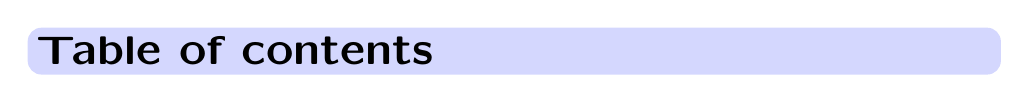
\begin{tikzpicture}
\node [fill=shade,rounded corners=5pt]
{
\begin{minipage}[t]{\textwidth}
\tableofcontents
\end{minipage}
};
\end{tikzpicture}
}
\titleformat{\section}{\Large\sf\bfseries\raggedright\color{headings}\thesection. }{}{0em}{}[\titlerule]


%%\maketitle
%%
%%%
%\labelofcontents
%%{
%\hypersetup{linkcolor=black}
%\tableofcontents
%}
%%
\hypertarget{synopsis}{%
\section{Synopsis}\label{synopsis}}

To inform the spatial component of the Darwin Harbour Sediment
Monitoring sampling design. In particular, to determine the `best'
location for 100 Sites in the East Arm and Outer Harbour sections of
Darwin Harbour.

To help inform this process, there are three broad sources of data
available:

\begin{enumerate}
\def\labelenumi{\arabic{enumi}.}
\item
  Hydrodynamic modelling of the entire Darwin Harbour. These data
  (availed via geoTiffs), comprise broadly tidal bed shear and velocity
  as well as wave driven forces at 10m resolution and will be used to
  isolate areas likely to experience deposition (rather than erosion) of
  sediments.
\item
  Munksgaard sediment chemical survey from 2012 provided by Lynda Radke
  (as an Excel workbook).\\
  These data provide background information that will be used to predict
  the full spatial distribution of a range of sediment chemicals. These
  spatial distributions will then help tune and evaluate a range of
  sampling designs.
\item
  Offset shallow Outer Harbour sediment survey provided by Lynda Radke
  (as an Excel workbook). Similar to the Munksgaard, data these data
  will provide background information for the Outer Harbour
\end{enumerate}

The basic procedure will involve the following steps:

\begin{enumerate}
\def\labelenumi{\arabic{enumi}.}
\tightlist
\item
  Read in a process the data sources
\item
  Fit a barrier spatial model to each of the Munksgaard sediment
  chemicals and predict/develop spatial layers for the East Arm section
\item
  Fit a barrier spatial model to each of the Offset shallow Outer
  Harbour sediment chemicals and predict/develop spatial layers for the
  Outer Harbour.
\item
  Develop masks out of the hydrodynamic model data and use them to
  exclude areas of likely erosion from the chemical spatial layers
\item
  Use spatial layers representing shipping channels, ports and other
  exclusion zones to establish additional masks to apply alongside
  hydrodynamic modelling masks to further restrict the sampling domains
  and prevent sampling configurations containing sites in the exclusion
  zones
\item
  Explore three different sample generation routines for a range of
  sample sizes to establish an optimal sampling design. The five
  routines will be:

  \begin{enumerate}
  \def\labelenumii{\alph{enumii})}
  \tightlist
  \item
    Using the masked chemical spatial layers to inform Conditioned
    Latent Hypercube Sampling - this will generate samples of nominated
    sizes that are located in a manner that most represents the
    underlying patterns in the chemical spatial layers.
  \item
    Completely random sampling - this will select the nominated number
    of samples from within the masked area and is completely naive to
    any underlying spatial patterns (and hence is only likely to be
    representative of the underlying patterns when the number of samples
    is large).
  \item
    A regular sampling grid - this will select approximately the
    nominated number of samples configured in a regular grid within the
    masked area. Like the completely random sampling, the regular
    sampling grid is completely naive to the underlying spatial
    patterns, yet it does guarantee a more even spatial coverage.
  \item
    A spatially balanced design - this will yield a spatially balanced
    design in which sampling sites are spread out throughout the spatial
    domain.
  \item
    A high dimensional spatially balanced design - this will yield a
    design in which sampling sites are spread in multiple dimensions
    (spatial and according to patterns in the underlying chemical
    distributions).
  \end{enumerate}
\end{enumerate}

In addition to the 100 long-term monitoring sites, there are 20 priority
sites. These sites are to be sampled more regularly and are for the
purpose of compliance monitoring specific areas. Although these sites
are additional to the long-term samples, they do form part of the
overall design and thus need to be considered when considering candidate
configurations.

All code for this project is available on github
\url{https://github.com/AIMS/darwin-harbour-sampling.git}

\hypertarget{data-processing}{%
\section{Data processing}\label{data-processing}}

\hypertarget{gis-data}{%
\subsection{GIS data}\label{gis-data}}

A shapefile of Darwin Harbour (see Figure \ref{fig:Map1}) will be
utilized in order to define the initial sampling domain(s). This project
will focus on the Outer Harbour and East Arm. For the purpose of the
sediment monitoring program, East Arm will be defined as East Arm,
Elizabeth River and a section of the Middle Harbour adjacent the city of
Darwin. The Outer Harbour will be defined as Outer Harbour and Shoal
Bay.

\begin{figure}
\centering\scriptsize
\includegraphics[width=0.7\textwidth,height=\textheight]{output/Map1.pdf}
\caption{Map of Darwin Harbour highlighting the Outer Harbour and East
Arm sections.\label{fig:Map1}}
\end{figure}

\hypertarget{munksgaard-2012-chemical-sediment-data}{%
\subsection{Munksgaard 2012 chemical sediment
data}\label{munksgaard-2012-chemical-sediment-data}}

Munksgaard 2012 chemical sediment data were provided by Lynda Radke in
the form of an Excel workbook. These data were consolidated together
into a single flat csv text file to support analyses. The spatial
configuration of the Munksgaard sediment sampling sites are illustrated
in Figure \ref{fig:Map2} (circular points). Primarily, only the sites
within the Outer Harbour and East Arm will be used to inform the current
exploration of future sampling designs.

Note, while the coverage of East Arm sites is extensive, the Outer
Harbour sites are clustered together in the south east corner of the
Outer Harbour (see Figure \ref{fig:Map2}). The use of these Munksgaard
2012 Outer Harbour sediment data to estimate the underlying patterns
throughout the entire Outer Harbour is not appropriate. Any modelling
patterns are only reliable within the spatial bounds of the available
data.\\
Any attempts to extrapolate to a broader area (e.g.~the rest of the
Outer Harbour), is not appropriate. Consequently, and unfortunately, the
Munksgaard sediment data is of little utility for designing a sampling
program for the Outer Harbour.

\hypertarget{offset-outer-harbour-sediment-monitoring-data}{%
\subsection{Offset Outer Harbour sediment monitoring
data}\label{offset-outer-harbour-sediment-monitoring-data}}

Offset Outer Harbour sediment monitoring data were provided by Lynda
Radke in the form of an Excel workbook. These data were consolidated
together into a single flat csv text file to support analyses. The
spatial configuration of the Offset Outer Harbour sediment sampling
sites are illustrated in Figure \ref{fig:Map2} (square ponts). These
data will be used to inform the selection of Outer Harbour sites.

\hypertarget{priority-sampling-sites}{%
\subsection{Priority sampling sites}\label{priority-sampling-sites}}

In addition to the long-term monitoring sites, a number of more
regularly sampled priority sites have been provided by Lynda Radke in
the form of an Excel workbook. These sites form additional sites, yet
must be considered in the formulation on site configurations and are
illustrated in Figure \ref{fig:Map2} as red points. Note, none of the
priority sites fall in the defined Outer Harbour and East Arms regions
and thus they will not be considered further.

\begin{figure}
\centering\scriptsize
\includegraphics[width=0.8\textwidth,height=\textheight]{output/Map2.pdf}
\caption{Map of Darwin Harbour indicating the spatial configuration of
Munksgaard 2012 sediment monitoring sites (dots). Solid dots signify
sites within the Outer Harbour and East Arm focal areas. Black circular
points represent Munksgaard 2012 sediment sampling sites, square points
represent Offset Outer Harbour sediment sites and red points represent
priority sites.\label{fig:Map2}}
\end{figure}

\newpage

\hypertarget{hydrodynamic-and-wave-modelling}{%
\subsection{Hydrodynamic and wave
modelling}\label{hydrodynamic-and-wave-modelling}}

When designing a sediment monitoring program, it is important to
consider the erosive, transportation and deposition forces operating on
the seabed. Ideally all, if not most, of the sampling sites should be
located in areas that are more likely to experience sediment deposition
than erosion or transportation.

Various hydrodynamic and wave modelling products were made available by
Dr.~Richard Brinkman (AIMS) that provide estimates of erosive,
transportation and deposition likelihoods and include:

\begin{itemize}
\tightlist
\item
  current velocity (50th and 75 percentiles - these are calculated from
  a 30 day characteristic spring-neap tidal cycle. Higher velocity
  equates to higher likelihood of sediment transport and erosion and
  thus lower probability of sediment deposition.
\item
  seabed shear stress (50th and 75 percentiles - these are derived from
  the current velocity and are a measure of the shear forces likely to
  be experienced on the sea bed due to tidal movement. Higher bed shear
  stress equates to higher likelihood of sediment transport and erosion
  and thus lower probability of sediment deposition.
\item
  wave derived orbital velocity magnitude at seabed - a shallow water
  wave model was applied using a 10 m/s wind forcing from a range of
  directions (0, 90, 140, 270 and 315 degrees) to simulate the likely
  orbital velocity experienced by the seabed. Higher orbital velocity
  equates to a higher likelihood of sediment transport and erosion and
  thus lower probability of sediment deposition.
\item
  wave derived seabed shear stress - the same shallow water wave model
  is expressed in terms of wave bed shear stress. Higher shear stress
  equates to higher likelihood of sediment transport and erosion and
  thus lower probability of sediment deposition.
\end{itemize}

Visual representations of each of the above products within the Outer
Harbour and East Arm focal areas are depicted in Figures
\ref{fig:hydro_outer} -- \ref{fig:waves_east}.

\begin{figure}
\centering\scriptsize
\includegraphics[width=1\textwidth,height=\textheight]{output/hydro_outer.png}
\caption{Outer Harbour extract of four hydrodynamic modeling tidal
products.\label{fig:hydro_outer}}
\end{figure}

\begin{figure}
\centering\scriptsize
\includegraphics[width=1\textwidth,height=\textheight]{output/hydro_east.png}
\caption{East Arm extract of four hydrodynamic modeling tidal
products.\label{fig:hydro_east}}
\end{figure}

\begin{figure}
\centering\scriptsize
\includegraphics[width=1\textwidth,height=\textheight]{output/waves_ubot_outer.png}
\caption{Outer Harbour extract of five hydrodynamic modeling wave
products. The different products represent different wind angles (0, 90,
140, 270 and 315 degrees).\label{fig:waves_outer}}
\end{figure}

\begin{figure}
\centering\scriptsize
\includegraphics[width=1\textwidth,height=\textheight]{output/waves_ubot_east.png}
\caption{East Arm extract of five hydrodynamic modeling wave products.
The different products represent different wind angles (0, 90, 140, 270
and 315 degrees).\label{fig:waves_east}}
\end{figure}

\hypertarget{masks}{%
\subsubsection{Masks}\label{masks}}

The seabed shear stress products provide spatial modelling of the
expected forces acting on the sea bed during a typical spring-neap tidal
cycle. In so doing, they provide proxies for the likelihood for sediment
erosion, transportation and deposition. These products can be used to
create masks that exclude areas of high erosive or transportation
potential.

To establish a mask (to focus only on deposition areas), thresholds need
to be established for what represent the critical values below which
deposition is likely. Figures \ref{fig:Hjulstroms} and
\ref{fig:shearStress} provide these for a range of sediment particle
sizes for water velocity and sea bed stress respectively.

\begin{figure}
\centering\scriptsize
\includegraphics[width=1\textwidth,height=\textheight]{data/Provided/hjulstrom.jpg}
\caption{Hjulstrom Curve linking sediment size and the velocity needed
to erode, transport or deposit (from
\url{https://www.thegeoroom.co.zw/hydrology/hjulstrom-curve.php}).\label{fig:Hjulstroms}}
\end{figure}

\begin{figure}
\centering\scriptsize
\includegraphics[width=0.6\textwidth,height=\textheight]{data/Provided/Critical-bed-shear-stress-C-for-erosion-of-continental-margin-particles-showing-the_W640.jpg}
\caption{Critical bed shear stress for erosion and particle settling
velocity of a range of particle sizes from Thomsen
(2002)\label{fig:shearStress}}
\end{figure}

\hypertarget{east-arm-sampling-domain}{%
\paragraph{East Arm sampling domain}\label{east-arm-sampling-domain}}

Figure \ref{fig:particle_sizes} illustrates the distribution of
percentage abundance of a range of particle sizes class categories from
the Munksgaard sampling program. On average, particles in the size
classes 4-62\(\mu\)m (Silt) and 62-250\(\mu\)m (fine sand) made up 25.4
and 43.4 percent of the sediment samples respectively. Hence, it is
important that future East Arm sampling designs focus on sites that will
ensure deposition of particles of these sizes. According to Figures
\ref{fig:Hjulstroms} and \ref{fig:shearStress}, particles at or above
29\(\mu\)m (middle of the silt range) correspond to critical deposition
values of approximately 0.2 m/s velocity and 0.1 seabed shear stress.

The hydrodynamic modeling seabed shear stress products represent the
50th and 75th percentile values. In the case of the 50th percentile,
this means that 50 percent of the time, seabed shear stress was
estimated to be above this value and 50 percent of values where below.
If a mask was based on setting the threshold to correspond to the 50th
percentile, then the masked layer represents areas where sediment
deposition is likely to occur more regularly than erosion and transport.

Nevertheless, it is important to also establish the distribution of
seabed shear stress across the seabed in order to better understand the
distribution of values. Figures \ref{fig:hist_hydro_east} and
\ref{fig:hist_waves_east} illustrate the frequency of seabed shear
stresses (and velocity) for the East Arm area. The 50th percentiles for
seabed shear stress appear to drop off the peak at around 0.2 m/s, hence
this appears to be a sensible threshold value.

\begin{figure}
\centering\scriptsize
\includegraphics[width=0.8\textwidth,height=\textheight]{output/particle_sizes.pdf}
\caption{The percentage abundance of different sediment grain sizes
observed across the Munksgaard sediment sampling
program.\label{fig:particle_sizes}}
\end{figure}

\begin{figure}
\centering\scriptsize
\includegraphics[width=0.8\textwidth,height=\textheight]{output/hist_hydro_east.pdf}
\caption{Frequency distributions of hydrodynamic products in the East
Arm area.\label{fig:hist_hydro_east}}
\end{figure}

\begin{figure}
\centering\scriptsize
\includegraphics[width=0.8\textwidth,height=\textheight]{output/hist_waves_east.pdf}
\caption{Frequency distributions of wave modelling seabed shear stress
products in the East Arm area.\label{fig:hist_waves_east}}
\end{figure}

Both current velocity and seabed shear stress are derived from the same
model and are thus closely correlated. Similarly, both wave derived
orbital velocity and wave derived seabed shear stress are correlated. In
each case, the shear stress proxies are intended to be expressions of
the forces that are likely to be acting on the seabed (from tides and
waves respectively). Hence, only the seabed shear stress versions of the
hydrodynamic and wave models will be used as the proxy estimates of
tidal and wave forces.

Figure \ref{fig:masks} illustrates the resulting masks for the East Arm
area using a threshold of 0.2 m/s (or 0.3 m/s for the 75th percentiles).
Each of the wave derived seabed shear masks were added together and then
joined with the 50 percentile hydrodynamic seabed shear mask. The
resulting mask is illustrated in Figure \ref{fig:mask_east}. This mask
represents (in blue shading) the areas most likely to experience more
deposition than erosion and thus suitable areas for sediment monitoring.
When we compare this mask to the spatial extent of the Munksgaard 2012
sediment monitoring site configuration, it is evident that while they
broadly overlap, there is substantially less suitable area in the region
adjacent to the City and substantially more in the East Arm reaches.

\begin{figure}
\centering\scriptsize
\includegraphics[width=0.9\textwidth,height=\textheight]{output/masks.png}
\caption{Individual East Arm masks from various hydrodynamic
(bedShear\_\emph{) and wave (beagle\_}) models categorised using a
threshold values of 0.2 for all other than the 75th percentile products
with use a threshold of 0.3 m/s. The blue areas indicate areas of
predicted relatively low erosion and transport potential and thus good
candidate areas for sample site allocation. The black dots illustrate
the position of Munksgaard 2012 sediment sampling
sites.\label{fig:masks}}
\end{figure}

\begin{figure}
\centering\scriptsize
\includegraphics[width=0.8\textwidth,height=\textheight]{output/masks1.png}
\caption{East Arm mask derived from the combination of 50th percentile
seabed shear stress and each of the wave derived seabed shear stresses.
The blue areas indicate areas of predicted relatively low erosion and
transport potential and thus good candidate areas for sample site
allocation. The black dots illustrate the position of Munksgaard 2012
sediment sampling sites.\label{fig:mask_east}}
\end{figure}

\hypertarget{outer-harbour-sampling-domain}{%
\subsection{Outer Harbour sampling
domain}\label{outer-harbour-sampling-domain}}

Figure \ref{fig:particle_sizes.outer} illustrates the distribution of
percentage abundance of a range of particle sizes class categories from
the Offsets Outer Harbour sampling program. The majority of particles
are classified as sand. Based on Figures \ref{fig:Hjulstroms} and
\ref{fig:shearStress}, it is likely that the majority of the sedient
particles are between 0.1mm and 1mm and that this corresponds to
critical deposition values of approximately 1 m/s to 5 m/s and 0.2-0.3
seabed shear stress.

\begin{figure}
\centering\scriptsize
\includegraphics[width=0.8\textwidth,height=\textheight]{output/particle_sizes.outer.pdf}
\caption{The percentage abundance of different sediment grain sizes
observed across the Offsets Outer Harbour sediment sampling
program.\label{fig:particle_sizes.outer}}
\end{figure}

The distribution of hydrodynamic seabed shear stress and velocity
(Figure \ref{fig:hist_hydro_outer}) has an initial valley at 0.3.\\
The distribution of wave derived seabed shear stress and velocity is
illustrated in Figure \ref{fig:hist_waves_outer}, however, and suggests
that the majority of the Outer Harbour is un-affected by high erosive
wave shear forces.

\begin{figure}
\centering\scriptsize
\includegraphics[width=0.8\textwidth,height=\textheight]{output/hist_hydro_outer.pdf}
\caption{Frequency distributions of hydrodynamic products in the Outer
Harbour area.\label{fig:hist_hydro_outer}}
\end{figure}

\begin{figure}
\centering\scriptsize
\includegraphics[width=0.8\textwidth,height=\textheight]{output/hist_waves_outer.pdf}
\caption{Frequency distributions of wave modelling seabed shear stress
products in the Outer Harbour area.\label{fig:hist_waves_outer}}
\end{figure}

\begin{figure}
\centering\scriptsize
\includegraphics[width=0.9\textwidth,height=\textheight]{output/masks_outer.png}
\caption{Individual Outer Harbour masks from various hydrodynamic
(bedShear\_\emph{) and wave (beagle\_}) models categorised using a
threshold values of 0.2 for all other than the 75th percentile products
with use a threshold of 0.3 m/s. The blue areas indicate areas of
predicted relatively low erosion and transport potential and thus good
candidate areas for sample site allocation. The black dots illustrate
the position of Munksgaard 2012 sediment sampling
sites.\label{fig:masks_outer}}
\end{figure}

A single combined mask, incorporating the 50th percentile seabed shear
stress and each of the wave derived seabed shear stresses is illustrated
in Figure \ref{fig:mask_outer} for Outer Harbour.

\begin{figure}
\centering\scriptsize
\includegraphics[width=0.8\textwidth,height=\textheight]{output/masks1_outer.png}
\caption{Outer Harbour mask derived from the combination of 50th
percentile seabed shear stress and each of the wave derived seabed shear
stresses. The blue areas indicate areas of predicted relatively low
erosion and transport potential and thus good candidate areas for sample
site allocation. The black dots illustrate the position of Munksgaard
2012 sediment sampling sites.\label{fig:mask_outer}}
\end{figure}

\hypertarget{exclusion-zone-masks}{%
\subsection{Exclusion zone masks}\label{exclusion-zone-masks}}

In addition to using hydrodynamic modelling masks to exclude areas that
might be considered unsuitable for sediment monitoring, there are areas
throughout Darwin Harbour that are not practical or appropriate for
monitoring. These include the shipping channel and port exclusion zones
as well as other exclusions zones associated with major infrastructure
of military bases. Hence additional masks were developed from spatial
layers provided by Lynda Radke. Maps

Figures \ref{fig:Map3a} and \ref{fig:Map3b} illustrate the sampling
masks associated with East Arm and Outer Harbour respectively.

\begin{figure}
\centering\scriptsize
\includegraphics[width=0.7\textwidth,height=\textheight]{output/Map3a.pdf}
\caption{East Arm mask derived from numerous exclusion zone shapefiles.
The blue areas represent the spatial domain avaialble for sampling. The
black dots illustrate the position of Munksgaard 2012 sediment sampling
sites. Red dots represent the priority sites. Open black and red circles
represent samples that are outside of the East Arm
area.\label{fig:Map3a}}
\end{figure}

\begin{figure}
\centering\scriptsize
\includegraphics[width=0.7\textwidth,height=\textheight]{output/Map3b.pdf}
\caption{Outer Harbour mask derived from numerous exclusion zone
shapefiles. The blue areas represent the spatial domain avaialble for
sampling. The black dots illustrate the position of Outer Harbour
sediment sampling sites. Open black circles represent samples that are
outside of the Outer Harbour area.\label{fig:Map3b}}
\end{figure}

\clearpage

\hypertarget{spatial-model-fitting}{%
\section{Spatial Model fitting}\label{spatial-model-fitting}}

A target or set of targets is required against which the effectiveness
and accuracy of candidate sampling designs can be tuned or gauged. This
target should represent the full underlying conditions and in essence
represent a saturated sampling design - a sampling design in which all
possible locations/sites are sampled. Whilst this is logistically not
possible, given an adequate set of baseline data, statistical spatial
models can be generated to estimate the underlying patterns. The
resulting predicted layers can be used to represent the targets.

Spatial models are complex statistical models that attempt to recreate
the full feature space from which a limited set of samples were
collected. In so doing, they attempt to incorporate two-dimensional
patterns and correlations to allow prediction to areas in between
samples.

In the simplest cases, simple surfaces can be derived by linear
interpolation between all the sampling points. However, when samples are
distributed unevenly, there are strong spatial dependencies and/or the
bounding domain is not a simple rectangle, more complex methodologies
are required.

Ecological and environmental process are often correlated through space.
To account for these spatial dependencies within a spatial model, it is
useful to incorporate a Gaussian Random Field (GRF) which specifies a
spatially dependent covariance structure in which locations that are
closer to one another in space will in general be more highly correlated
to one another than locations that are further apart.

Large or complex spatial models soon become intractable using a
traditional frequentist modelling framework. By contrast, equivalent
Bayesian models are typically very computationally expensive. Integrated
Nested Laplace Approximation (INLA: Rue, Martino, and Chopin 2009) is a
Bayesian approximation framework that offers the the philosophical
advantages of a full Bayesian approach, yet with the computational
efficiency of frequentist approaches.

We can consider a GRF to be stationary if the degree of correlation
between two points is dependent only on the distance between the points,
or non-stationary if we allow the correlation function to vary over the
landscape. An extreme form of non-stationary model occurs when there are
physical barriers that disrupt of block the flow of contagious
processes. In such cases, just because two locations are in close
proximity, does not necessarily mean that they will be highly
correlated. Consider a simple example of the diffusion of a dye in water
throughout a tank. The dye will spread out from the source and gradually
disperse throughout the tank. Consequently, the correlation between the
concentration of dye at any two locations during dispersion will be
dependent on the distance between the two locations. If however, the
tank had a partial barrier that restricted the flow of molecules, then
two locations either side of the barrier might have very different dye
concentrations despite being in close proximity. Barrier models are able
to account for these obstructions.

\[
\begin{align}
y_i &\sim{} \Gamma(\mu_i, \alpha)\\
log(\mu_i) &= \beta_0 + u(s_i) + \varepsilon_i\\[1em]
\beta_0 &\sim{} N(0,1000)\\
u(s_i) &\sim{} GRF(r, \sigma_u)\\ 
\varepsilon_i &\sim{} N(0, \sigma^2)\\[1em]
\pi(\sigma_e) &\sim{} \lambda_e e^{-\lambda_e \sigma_e}\\
\pi(\sigma_u) &\sim{} \lambda_0 e^{-\lambda_0 \sigma_u}\\
\pi\left(\frac{1}{r}\right) & \sim{} \lambda_1 e^{-\lambda_1 \frac{1}{r}}
\end{align}
\]

where \(y_i\) is the \(ith\) observation of the target chemical
variable, \(\varepsilon_i\) is the independent and individually variable
random effect used to model the very short range erratic dependencies
and \(u(s_i)\) is the Gaussian Random Field and is used to model the
long-range structural (autocorrelation) dependencies. A diffuse prior is
applied to the intercept (\(\beta_0\)) and \(\varepsilon_i\) a vector of
independent Gaussians. The Matern family spatial random effect
(\(u(s_i)\)) and its covariance is defined by two parameters: the range
(\(r\): represents the length scale of the spatial dependencies) and
standard deviation (\(\simga_u\): representing the ratio of spatial to
independent noise). The smaller the range, the lower the correlation
between two proximal locations.

In a boundary model, two different range parameters (\(r\)) are applied.
One of the range parameters is applied to the boundary area (in this
case land) and the other to the focal area (in this case Harbour). By
setting the boundary range smaller (and close to zero) than the focal
area range, the dependency structure across boundaries is disrupted and
approach zero.

Hyper-parameter priors for the random effects (\(\sigma_e\),
\(\sigma_u\)) as well as \(r\) are defined in terms of a \(\lambda\)
parameter which is determined by the scale of the response (on the log
scale in this case). Both \(\lambda_e\) and \(\lambda_0\) were set to
the median value of the target response (on a log scale). and the focal
area \(r\) was set to half the width of the spatial domain after (Bakka
et al. 2016).

The random field was approximated via a Constrained Refined Delaunay
Triangulation (CRDT) mesh. The mesh comprised of an inner region that
surrounded all the Munksgaard sediment monitoring sites as well as an
outer mesh provides a buffer to help ensure estimates close to the inner
mesh boundary are robust.\\
in doing so, the maximum permissible triangle edge length for the inner
and outer mesh regions was set to 0.01 and 0.04 (units of latlong
projection) respectively. The smaller the values, the finer the mesh.
This mesh is then projected onto the location of the observed sample
location.

The above models were fit for each of the sediment chemical recorded in
the Munksgaard 2012 sediment sampling program. Figure
\ref{fig:inla_model_east.arm_Mg} provides an example of the major
elements of one of the chemical (Magnesium) spatial models. Equivalent
figures for the other chemicals are presented in Appendix A. Figure
\ref{fig:inla_model_east.arm_Mg}a depicts the random field mesh with the
Muksgaard 2012 sampling sites and Harbour boundary overlayed. Figure
\ref{fig:inla_model_east.arm_Mg}b illustrates the boundary used for the
barrier in the spatial model and Figure
\ref{fig:inla_model_east.arm_Mg}c illustrates the final predicted
spatial layer (with original sample data overlayed) for Magnesium within
the East Arm area. For comparison, both predicted (model output) and
observed (Munksgaard samples) are presented on the same color scale.
Figure \ref{fig:inla_model_east.arm_Mg}c illustrates the final predicted
spatial layer for Magnesium within the East Arm area and where the color
scale is based purely on the range of predicted values.

\begin{figure}
\centering\scriptsize
\includegraphics[width=0.8\textwidth,height=\textheight]{output/inla_model_east.arm1_Mg.png}
\caption{Integrated Nested Laplace Approximation (INLA) barrier spatial
modelling of magnesium. The diagram illustrates a) the mesh, b) the
barrier mask, c) the resulting predicted 2D surface (and observed
training data as points) and d) the resulting predicted 2D surface
scaled to the range of predictions.\label{fig:inla_model_east.arm_Mg}}
\end{figure}

Although the shrinkage in models is a little high (there is a tendency
for the magnitude of change over space to be dampened), generally the
models do a very good job of depicting the relative patterns of change
in space. For this application, the absolute scale of the changes in
patterns are not important (only the relative patterns), since in order
to gauge the accuracy of any candidate sampling designs, it is necessary
to standardize the patterns anyway. So it is more important that the
model depict the general patterns in the observed data than the exact
values of the observed data.

\clearpage

\hypertarget{sampling}{%
\section{Sampling}\label{sampling}}

Ideally, a good sampling design should comprise of a configuration of
sites that collectively represent the broader area as efficiently as
possible. In this context, efficiency is a compromise between complete
representation (resulting from saturating the spatial domain with sites)
and minimizing sampling effort.

There are numerous approaches for generating candidate sampling
configurations. Irrespective of the approach, there must be a metric by
which the suitability of the configuration can be gauged. If we assume
that full saturation must provide maximum representation, then all other
configurations can be gauged relative to the full saturation.\\
Hence a measure of how well a configuration is likely to represent the
full spatial domain is the difference between some empirical property
calculated from the candidate configuration and full saturation. For
example, we could calculate the difference between the estimated mean
Magnesium from a candidate configuration and the equivalent mean
calculated from the full saturation. The magnitude of this difference is
thus a measure of the inaccuracy and thus suitability of the candidate
configuration.

In the current application, there are numerous sediment chemicals that
can be used to describe the underlying conditions within the spatial
domain. Consequently, the metric needs to incorporate the differences
across each of the chemicals. The following metric will be adopted.

\[
Mean Error = \frac{1}{n} \sum_{i=1:n}{\frac{abs(\bar{c_i} - \bar{s_i})}{\bar{r_i}}}
\]

\[
Max Error = \max_{i=1:n}{\frac{abs(\bar{c_i} - \bar{s_i})}{\bar{r_i}}}
\]

\[
Min Error = \min_{i=1:n}{\frac{abs(\bar{c_i} - \bar{s_i})}{\bar{r_i}}}
\]

where \(\bar{c}\) and \(\bar{s}\) are the estimated domain means of the
\(ith\) chemical (out of \(n\)) from the candidate and full saturation
configurations respectively and the normalizing constant (\(r_i\)) is
the difference between maximum and minimum predicted values for the
\(ith\) chemical. There are three metrics presented so capture three
broad characteristics of the `accuracy' of the candidate sampling
designs:

\begin{itemize}
\tightlist
\item
  MeanError - this is a measure of the average deviation between the
  estimated zone mean (from the candidate model) and target mean from
  across all chemical species.
\item
  MaxError - this is a measure of the maximum deviation between the
  estimated zone mean (from the candidate model) and the target mean
  from across all chemical species.\\
  As a maximum, it can be used to compare the worst performing aspects
  of each candidate and thus acts as a worst case scenario.
\item
  MinError - this is a measure of the minimum deviation between the
  estimated zone mean (from the candidate model) and the target mean
  from across all chemical species. As a minimum, it can be used to
  compare the best performing aspects of each candidate and thus acts as
  a best case scenario.
\end{itemize}

\hypertarget{random-sampling}{%
\paragraph{Random sampling}\label{random-sampling}}

The simplest approach to generating a spatial sampling design is to
repeatedly simulate sampling from the spatial domain with a range of
sample sizes and use the above metric to help determine the optimum
sampling size and configuration. Given a sufficiently large sample size,
random sampling should provide an unbiased and representative sampling
design. However, it is highly likely that at low sample sizes, this
approach will not yield highly representative samples (high \(Error\)),
yet, increasing the sample size should result (on average) in lower
\(Error\) (= greater accuracy). To counter the natural stochasticity
associated with simulation, we will repeat each sample size five times.

\hypertarget{sampling-on-a-regular-grid}{%
\paragraph{Sampling on a regular
grid}\label{sampling-on-a-regular-grid}}

In the simple random sampling approach above, each simulated random draw
is independent of all other draws. As a result, all configurations are
possible - even those in which multiple samples are aggregated together
in close proximity. In the absence of any prior knowledge about the
underlying environmental conditions and heterogeneity, an even and
regular spread of samples can ensure that the sampling design does offer
general representativeness. Grids of increasing sample size offer
progressively finer granularity and thus the ability to detect smaller
scale perturbations in space.

\hypertarget{conditioned-latin-hypercube-sampling}{%
\paragraph{Conditioned Latin Hypercube
Sampling}\label{conditioned-latin-hypercube-sampling}}

In drawing both random samples and regular grid samples, the process is
completely naive to the underlying environmental conditions.
Consequently, they will only likely to be representative once a large
number of samples have been collected. Conditional Latin Hypercube
Sampling (cLHS) is a robust and efficient statistical sampling procedure
that generates samples based on the variability within a
multidimensional covariate feature space (Minasny and McBratney 2006a).
Since the sampling process is supervised by the underlying conditions
(or proxies thereof), for a given sample size, the resulting candidate
sampling configurations are more likely to yield samples that are
representative of the complex underlying conditions.

In introducing the procedure, Minasny and McBratney (2006a) provided a
real world example of a soil mapping project in which relatively small
samples sizes generated by cLHS closely represented the original
distribution of a set of environmental covariates. Furthermore, Minasny
and McBratney (2006b) found cLHS superior (in terms of accuracy) to a
range of alternative sampling procedures including random and stratified
random sampling.

\hypertarget{spatially-balanced-design}{%
\paragraph{Spatially balanced design}\label{spatially-balanced-design}}

Whilst regular grid sampling designs do space samples out throughout the
spatial domain, they do have the potential to introduce biases due to
any underlying systematic processes that might align with the design
(albeit unintentionally) and do not necessarily provide good
representation.\\
On the other hand, random sampling designs offer some degree of
protection from those biases, the shear nature of randomization means
that it is possible that some sampling locations can be clustered in
very close proximity. When this is the case, not only does it waste
valuable sampling effort (as there is not need to provide multiple
estimates of the same location), it introduces another bias. Any
resulting estimates from the sampling design will be biased towards the
clustered sample conditions as those conditioned are effectively
weighted higher by virtue of the greater sampling effort.

The ideal design is to be able to have a random configuration that still
prevents the clustering of samples. In affect, a way to generate random
locations whose probability of selection is proportional to the distance
from all already selected sites. This is the inspiration behind
Spatially balanced designs.

There are numerous spatially balanced designed techniques. Some such as
Generalized Random-Tessellation Stratified (GRTS), map the full two
dimensional spatial domain into a single dimension (in a way that
preserves the spatial ordering) before applying a systematic \(\pi\)ps
sampling technique to ensure a balanced distribution of samples
throughout the spatial domain. Grafström, Lundström, and Schelin (2012)
introduced an alternative technique in which unequal inclusion
probabilities are generated via a pivotal method.

A further (and perhaps alternative) ideal is to be able to have a
balanced design not only based on spatial proximity, but also on the
basis of dissimilarity of underlying conditions. Spatial areas that are
homogeneous with respect to some underlying sampling conditions require
fewer sampling locations to characterize the underlying patterns than
areas that are relatively heterogeneous. The spatially balanced design
via pivotal method allows any number of dimensions to determine the
inclusion probabilities.

A key determinant of which of the above techniques to adopt is what the
purpose of the sampling design is for. If for example, the purpose is to
characterize the overal condition mean, then a 2D spatially balanced
design is arguably most appropriate as it should represent the general
underlying conditions. If on the other hand, the purpose is to be able
to model the underlying patterns and understand where any changes in
these patterns occur, then arguably a design that has been optimized
around the underlying conditions, such as a n-dimensional spatially
balanced design or conditioned latin hypercube sampling technique is
arguably more appropriate.

\hypertarget{east-arm}{%
\subsection{East Arm}\label{east-arm}}

For a range of sample sizes (5, 10, 20, 30, 40, 50, 60, 70, 80, 90, 100,
120, 200, 1000), for East Arm, each of the above sampling approaches was
repeated five times. For each run, the \(Error\) metric was calculated.
The results are presented in Figures \ref{fig:samplingEffort} (mean
error) and \ref{fig:samplingEffortMax} (max error). As expected. As the
sample sizes increase, the error declines. The simple random sampling
design performs worst. The regular grid sampling is better than the
random sampling. Whilst clusters of samples might be appropriate for
representing conditions when the conditions cluster correspondingly,
totally random samples are highly unlikely to resemble the correct
cluster configuration. The non uniform distribution of cLHS on the other
hand is directly due to the clustering patterns in the underlying
conditions and thus it is not surprising that this technique has the
least error.

Interestingly, the reduction in error after a sample size of 50 is
relatively mild (notwithstanding that the figure is presented on a log-y
scale). For each of sample sizes 50, 60, 70, 80 and 100, the best (based
on lowest error) cLHS configuration is presented in Figure.. Comma
delimeted text files are also available with the Latitude and Longitudes
of these coordinates.

\begin{figure}
\centering\scriptsize
\includegraphics[width=0.8\textwidth,height=\textheight]{output/SamplingEffort.pdf}
\caption{Comparison of the mean Error conditional on sample size and
sampling method for the East Arm\label{fig:samplingEffort}}
\end{figure}

\begin{figure}
\centering\scriptsize
\includegraphics[width=0.8\textwidth,height=\textheight]{output/SamplingEffortMax.pdf}
\caption{Comparison of the maximum Error conditional on sample size and
sampling method for the East Arm\label{fig:samplingEffortMax}}
\end{figure}

\begin{figure}
\centering\scriptsize
\includegraphics[width=0.8\textwidth,height=\textheight]{output/SamplingEffortMin.pdf}
\caption{Comparison of the minimum Error conditional on sample size and
sampling method for the East Arm\label{fig:samplingEffortMin}}
\end{figure}

On the basis of Figures \ref{fig:samplingEffort},
\ref{fig:samplingEffortMax} and \ref{fig:samplingEffortMin} we could
conclude that a sample size of 100 within East Arm is a sound choice,
although it is likely that as few as 50 could still potentially yield
similar overall patterns. The sample size of 100 also accommodates a
buffer against sample loss. Nevertheless, this entire simulation process
is contingent on a number of unverifiable assumptions:

\begin{enumerate}
\def\labelenumi{\arabic{enumi}.}
\tightlist
\item
  that the Munksgaard 2012 sediment sampling data are representative of
  the typical conditions and spatial patterns
\item
  all Munksgaard 2012 sediment chemicals are equally useful and
  informative
\item
  the INLA models are able to fully represent the true underlying
  conditions
\item
  the costs and logistics of sampling are equal irrespective of location
\end{enumerate}

The conditioned latin hypercube sampling technique consistently
outperforms the other techniques. Interestingly, there is very little
difference between the 2D and nD Spatially balanced designs. This
suggests that either the sediment chemicals are relatively homogeneous
over space or else patterns in one chemical species is countered by
patterns in another chemical species.

The conditioned latin hypercube sampling technique appears to be able to
tune its design on the underlying sediment chemical patterns better than
the spatially balanced designs. Thus if the above assumptions are
reasonable and the main intention of the sampling is to be able to
describe the patterns in the sediment chemicals, then the sampling
design derived from this technique would seem most appropriate.

If however, the purpose of the sampling design is be provide an unbiased
representative sample of the general conditions across the spatial
domain, then it could be argued that the 2D spatially balanced design is
most appropriate - particularly if there is any doubt in the above
assumptions.

\begin{figure}
\centering\scriptsize
\includegraphics[width=1\textwidth,height=\textheight]{output/SamplingDesign_clhs.pdf}
\caption{Sampling configurations associated with the lowest mean Error
for each sample size for cLHS for the East
Arm\label{fig:SamplingDesign_clhs}}
\end{figure}

\begin{figure}
\centering\scriptsize
\includegraphics[width=1\textwidth,height=\textheight]{output/SamplingDesign_regular.pdf}
\caption{Sampling configurations associated with the lowest mean Error
for each sample size for Regular grid sampling for the East
Arm\label{fig:SamplingDesign_regular}}
\end{figure}

\begin{figure}
\centering\scriptsize
\includegraphics[width=1\textwidth,height=\textheight]{output/SamplingDesign_spatiallybalanced2.pdf}
\caption{Sampling configurations associated with the lowest mean Error
for each sample size for nD Spatially balanced sampling for the East
Arm\label{fig:SamplingDesignspatiallybalanced2}}
\end{figure}

\begin{figure}
\centering\scriptsize
\includegraphics[width=1\textwidth,height=\textheight]{output/SamplingDesign_spatiallybalanced.pdf}
\caption{Sampling configurations associated with the lowest mean Error
for each sample size for 2D Spatially balanced sampling for the East
Arm\label{fig:SamplingDesignspatiallybalanced}}
\end{figure}

\begin{figure}
\centering\scriptsize
\includegraphics[width=1\textwidth,height=\textheight]{output/SamplingDesign_spatiallybalanced2_final.pdf}
\caption{Two dimensional spatially balanced sampling configuration for
the East Arm (100
samples)\label{fig:SamplingDesign_spatiallybalanced2_final}}
\end{figure}

\hypertarget{outer-harbour}{%
\subsection{Outer Harbour}\label{outer-harbour}}

For a range of sample sizes (5, 10, 20, 30, 40, 50, 60, 70, 80, 90, 100,
120, 200, 1000), for Outer Harbour, each of the above sampling
approaches was repeated five times. For each run, the \(Error\) metric
was calculated. The results are presented in Figures
\ref{fig:samplingEffort_outer} (mean error) and
\ref{fig:samplingEffortMax_outer} (max error). As expected. As the
sample sizes increase, the error declines. The simple random sampling
design performs worst. The regular grid sampling is better than the
random sampling. Whilst clusters of samples might be appropriate for
representing conditions when the conditions cluster correspondingly,
totally random samples are highly unlikely to resemble the correct
cluster configuration. The non uniform distribution of cLHS on the other
hand is directly due to the clustering patterns in the underlying
conditions and thus it is not surprising that this technique has the
least error.

Interestingly, the reduction in error after a sample size of 50 is
relatively mild (notwithstanding that the figure is presented on a log-y
scale). For each of sample sizes 50, 60, 70, 80 and 100, the best (based
on lowest error) cLHS configuration is presented in Figure.. Comma
delimeted text files are also available with the Latitude and Longitudes
of these coordinates.

\begin{figure}
\centering\scriptsize
\includegraphics[width=0.8\textwidth,height=\textheight]{output/SamplingEffort_outer.pdf}
\caption{Comparison of the mean Error conditional on sample size and
sampling method for the Outer Harbour\label{fig:samplingEffort_outer}}
\end{figure}

\begin{figure}
\centering\scriptsize
\includegraphics[width=0.8\textwidth,height=\textheight]{output/SamplingEffortMax_outer.pdf}
\caption{Comparison of the maximum Error conditional on sample size and
sampling method for the Outer
Harbour\label{fig:samplingEffortMax_outer}}
\end{figure}

\begin{figure}
\centering\scriptsize
\includegraphics[width=0.8\textwidth,height=\textheight]{output/SamplingEffortMin_outer.pdf}
\caption{Comparison of the minimum Error conditional on sample size and
sampling method for the Outer
Harbour\label{fig:samplingEffortMin_outer}}
\end{figure}

On the basis of Figures \ref{fig:samplingEffort_outer},
\ref{fig:samplingEffortMax_outer} and \ref{fig:samplingEffortMin_outer}
we could conclude that a sample size of 100 within Outer Harbour is a
sound choice, although it is likely that as few as 50 could still
potentially yield similar overall patterns. The sample size of 100 also
accommodates a buffer against sample loss. Nevertheless, this entire
simulation process is contingent on a number of unverifiable
assumptions:

\begin{enumerate}
\def\labelenumi{\arabic{enumi}.}
\tightlist
\item
  that the Offset Outer Harbour sediment sampling data are
  representative of the typical conditions and spatial patterns
\item
  all Offset Outer Harbour sediment chemicals are equally useful and
  informative
\item
  the INLA models are able to fully represent the true underlying
  conditions
\item
  the costs and logistics of sampling are equal irrespective of location
\end{enumerate}

Contrary to the situation for the East Arm area, the conditioned latin
hypercube sampling technique only outperforms the other techniques at
very low sample sizes. After a sample size of approximately 30, the 2D
spatially balanced design has better Minimum and Maximum Error. Also of
interest is the finding that the multidimensional spatially balanced
design is consistently worse than both a regular grid and 2D spatially
balanced design and on par with a totally random design. This might
suggest that there are fewer distinct patterns in the underlying
sediment chemical data as observed in the Offset Outer Harbour sampling
program.

Again, if however, the purpose of the sampling design is be provide an
unbiased representative sample of the general conditions across the
spatial domain, then it could be argued that the 2D spatially balanced
design is most appropriate - particularly if there is any doubt in the
above assumptions.

\begin{figure}
\centering\scriptsize
\includegraphics[width=1\textwidth,height=\textheight]{output/SamplingDesign_clhs_outer.pdf}
\caption{Sampling configurations associated with the lowest mean Error
for each sample size for cLHS for the Outer
Harbour\label{fig:SamplingDesign_clhs_outer}}
\end{figure}

\begin{figure}
\centering\scriptsize
\includegraphics[width=1\textwidth,height=\textheight]{output/SamplingDesign_regular_outer.pdf}
\caption{Sampling configurations associated with the lowest mean Error
for each sample size for Regular grid sampling for the Outer
Harbour\label{fig:SamplingDesign_regular_outer}}
\end{figure}

\begin{figure}
\centering\scriptsize
\includegraphics[width=1\textwidth,height=\textheight]{output/SamplingDesign_spatiallybalanced2_outer.pdf}
\caption{Sampling configurations associated with the lowest mean Error
for each sample size for nD Spatially balanced sampling for the Outer
Harbour\label{fig:SamplingDesign_spatiallybalanced2_outer}}
\end{figure}

\begin{figure}
\centering\scriptsize
\includegraphics[width=1\textwidth,height=\textheight]{output/SamplingDesign_spatiallybalanced_outer.pdf}
\caption{Sampling configurations associated with the lowest mean Error
for each sample size for 2D Spatially balanced sampling for the Outer
Harbour\label{fig:SamplingDesign_spatiallybalanced_outer}}
\end{figure}

\begin{figure}
\centering\scriptsize
\includegraphics[width=1\textwidth,height=\textheight]{output/SamplingDesign_spatiallybalanced2_final_outer.pdf}
\caption{Two dimensional spatially balanced sampling configuration for
the Outer Harbour (100
samples)\label{fig:SamplingDesign_spatiallybalanced2_final_outer}}
\end{figure}

\hypertarget{conclusions}{%
\section{Conclusions}\label{conclusions}}

Overall, 2D spatially balanced sampling designs for both Outer Harbour
and East Arm would seem most appropriate. These designs are immune to
any uncertainty in previous data and spatial modelling and should yield
well balanced spatial configurations. A total of 100 samples collected
from both East Arm and Outer Harbour is likely to yield representative
samples from which to construct a variety of spatio-temporal models into
the future.

\hypertarget{appendix-a}{%
\section{Appendix A}\label{appendix-a}}

\begin{figure}
\centering\scriptsize
\includegraphics[width=0.8\textwidth,height=\textheight]{output/inla_model_east.arm1_Al.png}
\caption{Integrated Nested Laplace Approximation (INLA) barrier spatial
modelling of Aluminium. The diagram illustrates a) the mesh, b) the
barrier mask, c) the resulting predicted 2D surface (and observed
training data as points) and d) the resulting predicted 2D surface
scaled to the range of predictions.\label{fig:inla_model_east.arm_Al}}
\end{figure}

\begin{figure}
\centering\scriptsize
\includegraphics[width=0.8\textwidth,height=\textheight]{output/inla_model_east.arm1_P.png}
\caption{Integrated Nested Laplace Approximation (INLA) barrier spatial
modelling of Phosphorus. The diagram illustrates a) the mesh, b) the
barrier mask, c) the resulting predicted 2D surface (and observed
training data as points) and d) the resulting predicted 2D surface
scaled to the range of predictions.\label{fig:inla_model_east.arm_P}}
\end{figure}

\begin{figure}
\centering\scriptsize
\includegraphics[width=0.8\textwidth,height=\textheight]{output/inla_model_east.arm1_S.png}
\caption{Integrated Nested Laplace Approximation (INLA) barrier spatial
modelling of Sulfur. The diagram illustrates a) the mesh, b) the barrier
mask, c) the resulting predicted 2D surface (and observed training data
as points) and d) the resulting predicted 2D surface scaled to the range
of predictions.\label{fig:inla_model_east.arm_S}}
\end{figure}

\begin{figure}
\centering\scriptsize
\includegraphics[width=0.8\textwidth,height=\textheight]{output/inla_model_east.arm1_Ca.png}
\caption{Integrated Nested Laplace Approximation (INLA) barrier spatial
modelling of Calcium. The diagram illustrates a) the mesh, b) the
barrier mask, c) the resulting predicted 2D surface (and observed
training data as points) and d) the resulting predicted 2D surface
scaled to the range of predictions.\label{fig:inla_model_east.arm_Ca}}
\end{figure}

\begin{figure}
\centering\scriptsize
\includegraphics[width=0.8\textwidth,height=\textheight]{output/inla_model_east.arm1_V.png}
\caption{Integrated Nested Laplace Approximation (INLA) barrier spatial
modelling of Vanadium. The diagram illustrates a) the mesh, b) the
barrier mask, c) the resulting predicted 2D surface (and observed
training data as points) and d) the resulting predicted 2D surface
scaled to the range of predictions.\label{fig:inla_model_east.arm_V}}
\end{figure}

\begin{figure}
\centering\scriptsize
\includegraphics[width=0.8\textwidth,height=\textheight]{output/inla_model_east.arm1_Cr.png}
\caption{Integrated Nested Laplace Approximation (INLA) barrier spatial
modelling of Chromium. The diagram illustrates a) the mesh, b) the
barrier mask, c) the resulting predicted 2D surface (and observed
training data as points) and d) the resulting predicted 2D surface
scaled to the range of predictions.\label{fig:inla_model_east.arm_Cr}}
\end{figure}

\begin{figure}
\centering\scriptsize
\includegraphics[width=0.8\textwidth,height=\textheight]{output/inla_model_east.arm1_Fe.png}
\caption{Integrated Nested Laplace Approximation (INLA) barrier spatial
modelling of Iron. The diagram illustrates a) the mesh, b) the barrier
mask, c) the resulting predicted 2D surface (and observed training data
as points) and d) the resulting predicted 2D surface scaled to the range
of predictions.\label{fig:inla_model_east.arm_Fe}}
\end{figure}

\begin{figure}
\centering\scriptsize
\includegraphics[width=0.8\textwidth,height=\textheight]{output/inla_model_east.arm1_Mn.png}
\caption{Integrated Nested Laplace Approximation (INLA) barrier spatial
modelling of Manganese. The diagram illustrates a) the mesh, b) the
barrier mask, c) the resulting predicted 2D surface (and observed
training data as points) and d) the resulting predicted 2D surface
scaled to the range of predictions.\label{fig:inla_model_east.arm_Mn}}
\end{figure}

\begin{figure}
\centering\scriptsize
\includegraphics[width=0.8\textwidth,height=\textheight]{output/inla_model_east.arm1_Co.png}
\caption{Integrated Nested Laplace Approximation (INLA) barrier spatial
modelling of Cobult. The diagram illustrates a) the mesh, b) the barrier
mask, c) the resulting predicted 2D surface (and observed training data
as points) and d) the resulting predicted 2D surface scaled to the range
of predictions.\label{fig:inla_model_east.arm_Co}}
\end{figure}

\begin{figure}
\centering\scriptsize
\includegraphics[width=0.8\textwidth,height=\textheight]{output/inla_model_east.arm1_Ni.png}
\caption{Integrated Nested Laplace Approximation (INLA) barrier spatial
modelling of Nickel. The diagram illustrates a) the mesh, b) the barrier
mask, c) the resulting predicted 2D surface (and observed training data
as points) and d) the resulting predicted 2D surface scaled to the range
of predictions.\label{fig:inla_model_east.arm_Ni}}
\end{figure}

\begin{figure}
\centering\scriptsize
\includegraphics[width=0.8\textwidth,height=\textheight]{output/inla_model_east.arm1_Cu.png}
\caption{Integrated Nested Laplace Approximation (INLA) barrier spatial
modelling of Copper. The diagram illustrates a) the mesh, b) the barrier
mask, c) the resulting predicted 2D surface (and observed training data
as points) and d) the resulting predicted 2D surface scaled to the range
of predictions.\label{fig:inla_model_east.arm_Cu}}
\end{figure}

\begin{figure}
\centering\scriptsize
\includegraphics[width=0.8\textwidth,height=\textheight]{output/inla_model_east.arm1_Zn.png}
\caption{Integrated Nested Laplace Approximation (INLA) barrier spatial
modelling of Zinc. The diagram illustrates a) the mesh, b) the barrier
mask, c) the resulting predicted 2D surface (and observed training data
as points) and d) the resulting predicted 2D surface scaled to the range
of predictions.\label{fig:inla_model_east.arm_Zn}}
\end{figure}

\begin{figure}
\centering\scriptsize
\includegraphics[width=0.8\textwidth,height=\textheight]{output/inla_model_east.arm1_Ga.png}
\caption{Integrated Nested Laplace Approximation (INLA) barrier spatial
modelling of Gallium. The diagram illustrates a) the mesh, b) the
barrier mask, c) the resulting predicted 2D surface (and observed
training data as points) and d) the resulting predicted 2D surface
scaled to the range of predictions.\label{fig:inla_model_east.arm_Ga}}
\end{figure}

\begin{figure}
\centering\scriptsize
\includegraphics[width=0.8\textwidth,height=\textheight]{output/inla_model_east.arm1_As.png}
\caption{Integrated Nested Laplace Approximation (INLA) barrier spatial
modelling of Arsenic. The diagram illustrates a) the mesh, b) the
barrier mask, c) the resulting predicted 2D surface (and observed
training data as points) and d) the resulting predicted 2D surface
scaled to the range of predictions.\label{fig:inla_model_east.arm_As}}
\end{figure}

\begin{figure}
\centering\scriptsize
\includegraphics[width=0.8\textwidth,height=\textheight]{output/inla_model_east.arm1_Se.png}
\caption{Integrated Nested Laplace Approximation (INLA) barrier spatial
modelling of Selenium. The diagram illustrates a) the mesh, b) the
barrier mask, c) the resulting predicted 2D surface (and observed
training data as points) and d) the resulting predicted 2D surface
scaled to the range of predictions.\label{fig:inla_model_east.arm_Se}}
\end{figure}

\begin{figure}
\centering\scriptsize
\includegraphics[width=0.8\textwidth,height=\textheight]{output/inla_model_east.arm1_Mo.png}
\caption{Integrated Nested Laplace Approximation (INLA) barrier spatial
modelling of Molybdenum. The diagram illustrates a) the mesh, b) the
barrier mask, c) the resulting predicted 2D surface (and observed
training data as points) and d) the resulting predicted 2D surface
scaled to the range of predictions.\label{fig:inla_model_east.arm_Mo}}
\end{figure}

\begin{figure}
\centering\scriptsize
\includegraphics[width=0.8\textwidth,height=\textheight]{output/inla_model_east.arm1_Ca.png}
\caption{Integrated Nested Laplace Approximation (INLA) barrier spatial
modelling of Cadmium. The diagram illustrates a) the mesh, b) the
barrier mask, c) the resulting predicted 2D surface (and observed
training data as points) and d) the resulting predicted 2D surface
scaled to the range of predictions.\label{fig:inla_model_east.arm_Ca}}
\end{figure}

\begin{figure}
\centering\scriptsize
\includegraphics[width=0.8\textwidth,height=\textheight]{output/inla_model_east.arm1_Pb.png}
\caption{Integrated Nested Laplace Approximation (INLA) barrier spatial
modelling of Lead. The diagram illustrates a) the mesh, b) the barrier
mask, c) the resulting predicted 2D surface (and observed training data
as points) and d) the resulting predicted 2D surface scaled to the range
of predictions.\label{fig:inla_model_east.arm_Pb}}
\end{figure}

\hypertarget{appendix-b}{%
\section{Appendix B}\label{appendix-b}}

\begin{figure}
\centering\scriptsize
\includegraphics[width=0.8\textwidth,height=\textheight]{output/inla_model_outer1_Al.png}
\caption{Integrated Nested Laplace Approximation (INLA) barrier spatial
modelling of Aluminium. The diagram illustrates a) the mesh, b) the
barrier mask, c) the resulting predicted 2D surface (and observed
training data as points) and d) the resulting predicted 2D surface
scaled to the range of predictions.\label{fig:inla_model_outer_Al}}
\end{figure}

\begin{figure}
\centering\scriptsize
\includegraphics[width=0.8\textwidth,height=\textheight]{output/inla_model_outer1_As.png}
\caption{Integrated Nested Laplace Approximation (INLA) barrier spatial
modelling of Arsenic. The diagram illustrates a) the mesh, b) the
barrier mask, c) the resulting predicted 2D surface (and observed
training data as points) and d) the resulting predicted 2D surface
scaled to the range of predictions.\label{fig:inla_model_outer_As}}
\end{figure}

\begin{figure}
\centering\scriptsize
\includegraphics[width=0.8\textwidth,height=\textheight]{output/inla_model_outer1_Ce.png}
\caption{Integrated Nested Laplace Approximation (INLA) barrier spatial
modelling of Cerium. The diagram illustrates a) the mesh, b) the barrier
mask, c) the resulting predicted 2D surface (and observed training data
as points) and d) the resulting predicted 2D surface scaled to the range
of predictions.\label{fig:inla_model_outer_Ce}}
\end{figure}

\begin{figure}
\centering\scriptsize
\includegraphics[width=0.8\textwidth,height=\textheight]{output/inla_model_outer1_Cr.png}
\caption{Integrated Nested Laplace Approximation (INLA) barrier spatial
modelling of Cromium. The diagram illustrates a) the mesh, b) the
barrier mask, c) the resulting predicted 2D surface (and observed
training data as points) and d) the resulting predicted 2D surface
scaled to the range of predictions.\label{fig:inla_model_outer_Cr}}
\end{figure}

\begin{figure}
\centering\scriptsize
\includegraphics[width=0.8\textwidth,height=\textheight]{output/inla_model_outer1_Cu.png}
\caption{Integrated Nested Laplace Approximation (INLA) barrier spatial
modelling of Copper. The diagram illustrates a) the mesh, b) the barrier
mask, c) the resulting predicted 2D surface (and observed training data
as points) and d) the resulting predicted 2D surface scaled to the range
of predictions.\label{fig:inla_model_outer_Cu}}
\end{figure}

\begin{figure}
\centering\scriptsize
\includegraphics[width=0.8\textwidth,height=\textheight]{output/inla_model_outer1_Fe.png}
\caption{Integrated Nested Laplace Approximation (INLA) barrier spatial
modelling of Iron. The diagram illustrates a) the mesh, b) the barrier
mask, c) the resulting predicted 2D surface (and observed training data
as points) and d) the resulting predicted 2D surface scaled to the range
of predictions.\label{fig:inla_model_outer_Fe}}
\end{figure}

\begin{figure}
\centering\scriptsize
\includegraphics[width=0.8\textwidth,height=\textheight]{output/inla_model_outer1_Mn.png}
\caption{Integrated Nested Laplace Approximation (INLA) barrier spatial
modelling of Manganese. The diagram illustrates a) the mesh, b) the
barrier mask, c) the resulting predicted 2D surface (and observed
training data as points) and d) the resulting predicted 2D surface
scaled to the range of predictions.\label{fig:inla_model_outer_Mn}}
\end{figure}

\begin{figure}
\centering\scriptsize
\includegraphics[width=0.8\textwidth,height=\textheight]{output/inla_model_outer1_Ni.png}
\caption{Integrated Nested Laplace Approximation (INLA) barrier spatial
modelling of Nickel. The diagram illustrates a) the mesh, b) the barrier
mask, c) the resulting predicted 2D surface (and observed training data
as points) and d) the resulting predicted 2D surface scaled to the range
of predictions.\label{fig:inla_model_outer_Ni}}
\end{figure}

\begin{figure}
\centering\scriptsize
\includegraphics[width=0.8\textwidth,height=\textheight]{output/inla_model_outer1_Pb.png}
\caption{Integrated Nested Laplace Approximation (INLA) barrier spatial
modelling of Lead. The diagram illustrates a) the mesh, b) the barrier
mask, c) the resulting predicted 2D surface (and observed training data
as points) and d) the resulting predicted 2D surface scaled to the range
of predictions.\label{fig:inla_model_outer_Pb}}
\end{figure}

\begin{figure}
\centering\scriptsize
\includegraphics[width=0.8\textwidth,height=\textheight]{output/inla_model_outer1_Sb.png}
\caption{Integrated Nested Laplace Approximation (INLA) barrier spatial
modelling of Antonium. The diagram illustrates a) the mesh, b) the
barrier mask, c) the resulting predicted 2D surface (and observed
training data as points) and d) the resulting predicted 2D surface
scaled to the range of predictions.\label{fig:inla_model_outer_Sb}}
\end{figure}

\begin{figure}
\centering\scriptsize
\includegraphics[width=0.8\textwidth,height=\textheight]{output/inla_model_outer1_V.png}
\caption{Integrated Nested Laplace Approximation (INLA) barrier spatial
modelling of Vanadium. The diagram illustrates a) the mesh, b) the
barrier mask, c) the resulting predicted 2D surface (and observed
training data as points) and d) the resulting predicted 2D surface
scaled to the range of predictions.\label{fig:inla_model_outer_V}}
\end{figure}

\begin{figure}
\centering\scriptsize
\includegraphics[width=0.8\textwidth,height=\textheight]{output/inla_model_outer1_Zn.png}
\caption{Integrated Nested Laplace Approximation (INLA) barrier spatial
modelling of Zn. The diagram illustrates a) the mesh, b) the barrier
mask, c) the resulting predicted 2D surface (and observed training data
as points) and d) the resulting predicted 2D surface scaled to the range
of predictions.\label{fig:inla_model_outer_Zn}}
\end{figure}

\begin{figure}
\centering\scriptsize
\includegraphics[width=0.8\textwidth,height=\textheight]{output/inla_model_outer1_TOC.png}
\caption{Integrated Nested Laplace Approximation (INLA) barrier spatial
modelling of Total organic Carbon. The diagram illustrates a) the mesh,
b) the barrier mask, c) the resulting predicted 2D surface (and observed
training data as points) and d) the resulting predicted 2D surface
scaled to the range of predictions.\label{fig:inla_model_outer_TOC}}
\end{figure}

\begin{figure}
\centering\scriptsize
\includegraphics[width=0.8\textwidth,height=\textheight]{output/inla_model_outer1_TN.png}
\caption{Integrated Nested Laplace Approximation (INLA) barrier spatial
modelling of Total Nitrogen. The diagram illustrates a) the mesh, b) the
barrier mask, c) the resulting predicted 2D surface (and observed
training data as points) and d) the resulting predicted 2D surface
scaled to the range of predictions.\label{fig:inla_model_outer_TN}}
\end{figure}

This document was produced from markdown using knitr on R version 3.6.0
(2019-04-26) on a x86\_64-pc-linux-gnu system.

\begin{Shaded}
\begin{Highlighting}[]
\OperatorTok{>}\StringTok{ }\KeywordTok{sessionInfo}\NormalTok{()}
\end{Highlighting}
\end{Shaded}

\begin{verbatim}
R version 3.6.0 (2019-04-26)
Platform: x86_64-pc-linux-gnu (64-bit)
Running under: ArcoLinux

Matrix products: default
BLAS:   /usr/lib/libopenblasp-r0.3.5.so
LAPACK: /usr/lib/liblapack.so.3.8.0

locale:
 [1] LC_CTYPE=en_AU.utf8        LC_NUMERIC=C               LC_TIME=en_AU.UTF-8       
 [4] LC_COLLATE=en_AU.utf8      LC_MONETARY=en_AU.UTF-8    LC_MESSAGES=en_AU.utf8    
 [7] LC_PAPER=en_AU.UTF-8       LC_NAME=C                  LC_ADDRESS=C              
[10] LC_TELEPHONE=C             LC_MEASUREMENT=en_AU.UTF-8 LC_IDENTIFICATION=C       

attached base packages:
[1] stats     graphics  grDevices utils     datasets  methods   base     

other attached packages:
[1] knitr_1.22

loaded via a namespace (and not attached):
[1] compiler_3.6.0 magrittr_1.5   tools_3.6.0    stringi_1.4.3  stringr_1.4.0  xfun_0.6      
[7] evaluate_0.13 
\end{verbatim}

\hypertarget{references}{%
\section*{References}\label{references}}
\addcontentsline{toc}{section}{References}

\hypertarget{refs}{}
\leavevmode\hypertarget{ref-Bakka-2016-1608}{}%
Bakka, Haakon, Jarno Vanhatalo, Janine Illian, Daniel Simpson, and
Håvard Rue. 2016. ``Non-stationary Gaussian models with physical
barriers.'' \emph{arXiv E-Prints}, August, arXiv:1608.03787.
\url{http://arxiv.org/abs/1608.03787}.

\leavevmode\hypertarget{ref-Grafstrom-2012}{}%
Grafström, Anton, Niklas L. P. Lundström, and Lina Schelin. 2012.
``Spatially Balanced Sampling Through the Pivotal Method.''
\emph{Biometrics} 68 (2): 514--20.
\url{https://doi.org/10.1111/j.1541-0420.2011.01699.x}.

\leavevmode\hypertarget{ref-Minasny-2006-1378}{}%
Minasny, B., and A. B. McBratney. 2006a. ``A Conditioned Latin Hypercube
Method for Sampling in the Presence of Ancillary Information.''
\emph{Computers \& Geosciences} 32 (9): 1378--88.
\url{https://doi.org/https://doi.org/10.1016/j.cageo.2005.12.009}.

\leavevmode\hypertarget{ref-Minasny-2006-153}{}%
---------. 2006b. ``Chapter 12 Latin Hypercube Sampling as a Tool for
Digital Soil Mapping.'' In \emph{Digital Soil Mapping}, edited by P.
Lagacherie, A. B. McBratney, and M. Voltz, 31:153--606. Developments in
Soil Science. Elsevier.
\url{https://doi.org/https://doi.org/10.1016/S0166-2481(06)31012-4}.

\leavevmode\hypertarget{ref-Rue-2009-319}{}%
Rue, H., S. Martino, and N. Chopin. 2009. ``Approximate Bayesian
Inference for Latent Gaussian Models Using Integrated Nested Laplace
Approximations.'' \emph{Journal of the Royal Society of Statistics
Series B - Statistical Methodology} 71 (2): 319--92.

\leavevmode\hypertarget{ref-Thomsen-2002-2002}{}%
Thomsen, Laurenz. 2002. ``The Benthic Boundary Layer.'' In, 143--55.
\url{https://doi.org/10.1007/978-3-662-05127-6_9}.
%

%\addcontentsline{toc}{section}{References and additional reading}\titleformat{\section}{\Large\sf\bfseries\raggedright\color{headings}}{}{0em}{}[\titlerule]

%%%
%%
\end{document}
